\documentclass[11pt]{article}
\usepackage[margin=1.05in]{geometry}
\usepackage{amsmath,amssymb}
\usepackage{booktabs}
\usepackage{tikz}
\usetikzlibrary{positioning}
\usepackage[hidelinks]{hyperref}
\usepackage{parskip}

\newcommand{\CNOT}{\textsc{cnot}}
\newcommand{\CCNOT}{\textsc{ccnot}}
\newcommand{\code}[1]{\texttt{#1}}
\newcommand{\xor}{\mathbin{\hat{}}\mathord{=}}

\title{\textbf{The Balanced Sliced Sandwich}\\[2pt]
\large Construction, slice contract, and how to select it}
\author{local\_mixing project}
\date{September 5, 2026 \\ \small branch \code{drip-reshuffle}, commit \code{b38a438f}}

\begin{document}
\maketitle

\begin{abstract}
\noindent The \emph{balanced} sliced sandwich is a variant of the sliced
sandwich in which each half of the $2n$ wires hosts one computation, rather
than both computations sharing the low half. It is selected per run --- never
per build --- and the default everywhere is the original (\emph{classic})
construction. This note summarises what changes, why one further change is
forced, what the resulting slice contract is in both directions, and how to
ask for it. Full spec of both variants: \code{docs/SLICED\_SANDWICH.\{md,tex,pdf\}}.
\end{abstract}

\section{The option}

The choice bit is \code{SandwichVariant}, defaulting to \code{Classic}. Three
equivalent ways to ask for the balanced construction, all decided when the tool
runs:

\begin{center}
\begin{tabular}{ll}
\toprule
entry point & selector \\
\midrule
mixing driver & \code{sss --cnot --sliced-sandwich {-}{-}sandwich-balanced \dots} \\
pipeline binary & \code{gen\_sandwich\_gadget \dots\ <gadgetization\_mode> <sandwich\_variant>} \\
pipeline binary & \code{SANDWICH\_VARIANT=classic|balanced} (positional wins) \\
library & \code{sliced\_sandwich\_cnot(\dots, SandwichVariant::Balanced, rng)} \\
\bottomrule
\end{tabular}
\end{center}

\noindent Classic output is unchanged by the addition: the builder draws the
same values in the same order as before, so any classic seed still reproduces
its circuit bit for bit.

\section{What changes}

Two changes, exactly as specified, plus one that the algebra forces.

\begin{enumerate}
\item The copy step flips direction: $N: x \xor y$ (wire $i \xor$ wire $n{+}i$)
      instead of $y \xor x$.
\item The $D$ block moves to the second half, $D'$ on wires $n..2n{-}1$.
\item \emph{Forced:} the second slice block mirrors with $D$ --- $S_2'$ targets
      the second half and reads the first,
      \[
        \underbrace{y_i \xor x_j}_{\text{\CNOT, }\approx 1/3}
        \qquad
        \underbrace{y_i \xor y_j \wedge x_k}_{\text{\CCNOT, rest}}
      \]
      so it is dead when the \emph{first} half is zero.
\end{enumerate}

\noindent $C$, $S_1$, the random interleaving and the float stage are
untouched. So
\[
\text{classic:}\quad A = [\, C \parallel S_1 \,];\; N(y \xor x);\; [\, D \parallel S_2 \,]
\]
\[
\text{balanced:}\quad A = [\, C \parallel S_1 \,];\; N(x \xor y);\; [\, D' \parallel S_2' \,]
\]
with the same size, $\lvert C\rvert + m + n + 2s$ gates on $2n$ wires.

\begin{figure}[h]
\centering
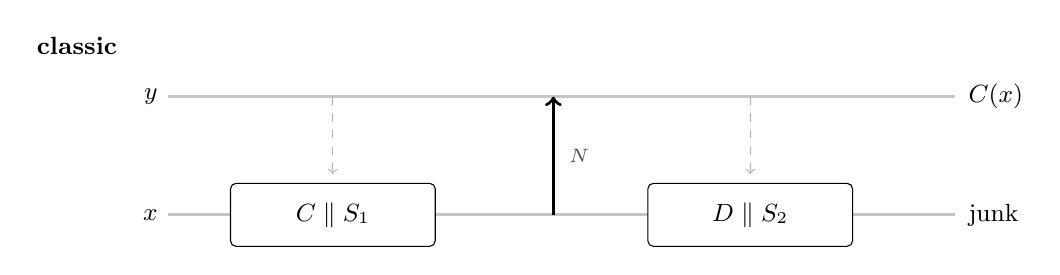
\begin{tikzpicture}[
  lane/.style={very thick, gray!45},
  blk/.style={draw, rounded corners=2pt, minimum height=8mm, minimum width=26mm,
              fill=white, font=\small, inner sep=2pt},
  rd/.style={->, dashed, gray!65, shorten >=2pt},
  nn/.style={->, very thick},
  lbl/.style={font=\scriptsize\itshape, gray!60!black}
]
% ---------------- classic ----------------
\node[font=\bfseries\small] at (-1.15,2.15) {classic};
\draw[lane] (0,1.5) -- (10,1.5);
\draw[lane] (0,0) -- (10,0);
\node[left, font=\small] at (0,1.5) {$y$};
\node[left, font=\small] at (0,0) {$x$};
\node[blk] at (2.1,0) {$C \parallel S_1$};
\node[blk] at (7.4,0) {$D \parallel S_2$};
\draw[rd] (2.1,1.5) -- (2.1,0.45);
\draw[rd] (7.4,1.5) -- (7.4,0.45);
\draw[nn] (4.9,0) -- (4.9,1.5);
\node[lbl, right] at (4.98,0.75) {$N$};
\node[right, font=\small] at (10.05,1.5) {$C(x)$};
\node[right, font=\small] at (10.05,0) {junk};
\end{tikzpicture}

\vspace{5mm}

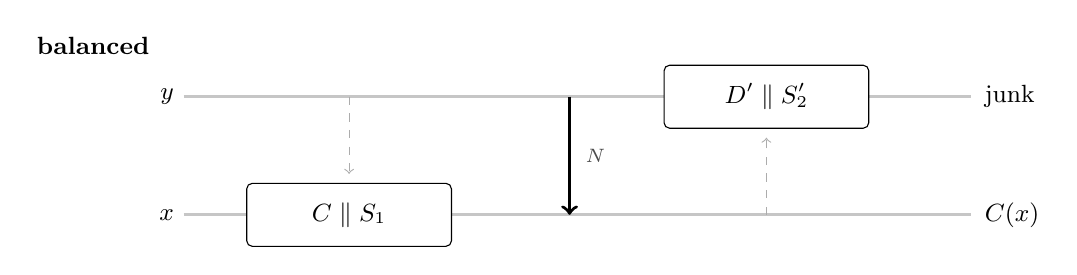
\begin{tikzpicture}[
  lane/.style={very thick, gray!45},
  blk/.style={draw, rounded corners=2pt, minimum height=8mm, minimum width=26mm,
              fill=white, font=\small, inner sep=2pt},
  rd/.style={->, dashed, gray!65, shorten >=2pt},
  nn/.style={->, very thick},
  lbl/.style={font=\scriptsize\itshape, gray!60!black}
]
% ---------------- balanced ----------------
\node[font=\bfseries\small] at (-1.15,2.15) {balanced};
\draw[lane] (0,1.5) -- (10,1.5);
\draw[lane] (0,0) -- (10,0);
\node[left, font=\small] at (0,1.5) {$y$};
\node[left, font=\small] at (0,0) {$x$};
\node[blk] at (2.1,0) {$C \parallel S_1$};
\node[blk] at (7.4,1.5) {$D' \parallel S_2'$};
\draw[rd] (2.1,1.5) -- (2.1,0.45);
\draw[rd] (7.4,0) -- (7.4,1.05);
\draw[nn] (4.9,1.5) -- (4.9,0);
\node[lbl, right] at (4.98,0.75) {$N$};
\node[right, font=\small] at (10.05,1.5) {junk};
\node[right, font=\small] at (10.05,0) {$C(x)$};
\end{tikzpicture}
\caption{Solid arrow: the copy step $N$. Dashed arrows: a slice block reading
the opposite half (dead when that half is zero). Outputs shown for the forward
zero slice $y=0$. In classic both computations live on $x$ and the answer is
copied up into a pure register; in balanced each half hosts one computation and
the answer never moves.}
\end{figure}

\section{Why $S_2$ must mirror}

With $D'$ on the second half, a low-targeting $S_2$ would fire as soon as $D'$
makes the second half nonzero, and it would overwrite the forward answer, which
in this layout stays in the \emph{first} half. Mirroring $S_2$ with $D$ is
therefore what restores a slice contract, and it lands the block exactly where
the inverse direction needs it: dead on $x=0$.

The general rule --- satisfied by both variants --- is:

\begin{center}
\begin{tabular}{lccc}
\toprule
block & fires in & targets & that half is \\
\midrule
$S_1$ (both variants) & inverse & low  & inverse junk \\
$S_2$  classic        & forward & low  & forward junk \\
$S_2'$ balanced       & forward & \textbf{high} & forward junk \\
\bottomrule
\end{tabular}
\end{center}

\noindent Each slice block is dead in one direction and fires in the other, and
when it fires it only ever hits that direction's junk half. $S_1$ needs no
change because its role is unchanged; $S_2$ flips because moving $D$ moved the
forward-junk half.

\section{Slice contract}

\subsection*{Forward, on $y=0$: the answer is the low half}

\[
(x,0)
\xrightarrow{\;C \parallel S_1\;} (C(x),\,0)
\xrightarrow{\;N\;} (C(x),\,0)
\xrightarrow{\;D' \parallel S_2'\;} (C(x),\,\text{junk})
\]
$S_1$ is dead through the $C$ stage (nothing writes the second half before
$N$), the flipped copy step is a no-op on the slice, and block 2 writes only
the second half --- so the answer is frozen where block 1 left it:
\[
\boxed{\;A(x,0) = (C(x),\,\text{junk})\;}
\]
Where classic protects the answer by moving it into a register the second block
never targets, balanced protects it by leaving it in a half the second block
never targets.

\subsection*{Inverse, on the mirrored slice $x=0$: the answer is the high half}

\[
(0,q)
\xrightarrow{\;(D' \parallel S_2')^{-1}\;} (0,\,D^{-1}(q))
\xrightarrow{\;N\;} (D^{-1}(q),\,D^{-1}(q))
\xrightarrow{\;(C \parallel S_1)^{-1}\;} (\text{junk},\,D^{-1}(q))
\]
$S_2'$ is dead because the first half is zero, so $D^{-1}$ computes cleanly;
$N$ copies it down; and the reversed block 1 --- $C^{-1}$ with $S_1$ now firing
on a nonzero second half --- junks the first half only:
\[
\boxed{\;A^{-1}(0,q) = (\text{junk},\, D^{-1}(q))\;}
\]

\subsection*{Off-slice}

For $y \neq 0$ the first-half output is $C'(x,y) \oplus y$, where $C'$ is the
$S_1$-disturbed computation. The flipped copy step supplies exactly the same
$y\oplus$ masking as the classic one, now on the answer half, so no nonzero
slice yields the clean answer.

\section{What balance buys, and what it costs}

Each half is one direction's computation lane and the other direction's answer:
$C$ owns the first half, $D$ the second. The two directions therefore have
\emph{different} slices --- $y=0$ forward, $x=0$ backward --- where the classic
construction slices both at $y=0$ and reads both out on the high half.
Equivalently: classic has a half (the low one) that is junk in \emph{both}
directions; balanced has none, since every half is somebody's payload.

One asymmetry comes with it. On the forward slice the $D'$ lane starts from the
constant $0$ rather than from live data, so its junk output depends on $x$ only
through the $S_2'$ injections; the classic layout's junk half instead starts
from $C(x)$ and runs $D$ on it.

\section{Verification}

The driver pins the balanced contract through the \code{SandwichFirst} function
view --- second half of the input forced to zero, first-half output must equal
$C(x)$ --- checked after the transform and after every mixing round. Unit tests
cover the mirrored slice block's deadness on $x=0$, the forward contract with a
permutation check, and the inverse's exact recovery of $D^{-1}$ on the mirrored
slice (testing $D(D^{-1}(q)) = q$ against the explicit $D$, not merely
bijectivity); the float-band regression test runs over both variants. The
classic path was additionally checked gate for gate, and rng-state for
rng-state, against the pre-variant builder over $n \in \{3,5,8,16\}$ and $24$
seeds.

\vspace{4pt}
\noindent\textbf{Provenance.} \code{SandwichVariant}, \code{sliced\_sandwich\_cnot},
\code{sliced\_sandwich\_with\_d}, \code{sliced\_sandwich\_build},
\code{sandwich\_slice\_gates}, \code{shift\_xgate\_wires} in
\code{src/preprocessing/gadgets.rs}; \code{FunctionView::SandwichFirst} and
\code{sandwich\_balanced} in \code{src/db\_mixing/main\_mix\_cnot.rs}; flags in
\code{src/main.rs} and \code{src/commands/sss.rs}; variant argument and
\code{SANDWICH\_VARIANT} in
\code{src/preprocessing/bin/gen\_sandwich\_gadget.rs}.

\end{document}
